\subsubsection{ANDES}

\subsubsection{Test case: Kundur two-area system}

The Kundur two-area system is a standard benchmark network widely used for small-signal and transient stability studies. It was introduced in the P. Kundur power system stability literature as a compact, yet representative, test case that exposes inter-area oscillatory modes and control interactions without excessive model complexity.

\begin{figure}[h!]
    \centering
    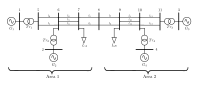
\includegraphics[width=1\linewidth]{figures/Kundur_system_no_shunt.pdf}
    \caption{Kundur two area system without shunt.}
    \label{fig:kundur_system}
\end{figure}

The main characteristics of the system, depicted in Figure \ref{fig:kundur_system}, are:
\begin{itemize}
    \item Two areas connected by a pair of parallel lines. In each area, 2 synchronous generators are placed so that each area can swing against each other and produce inter-area oscillations.
    \item All the synchronous generators are connected to the network through a transformer.
    \item In this version of the Kundur two-area system no shunts are connected to buses 7 and 9.
    \item The base power is 100 MW and the voltage levels are 20kV for the generators and 230kV for the network.
\end{itemize}

The following code can be used to model the Kundur two area system without shunt in VeraGrid and to perform the small-signal Stability analysis. As seen in the code, an event is created at time instant 2.5s where the active power of load A is increased to 900MW.